\documentclass[preprint,nocopyrightspace]{sigplanconf}

\usepackage{color}
\usepackage{listings}
\definecolor{StringRed}{rgb}{.637,0.082,0.082}
\definecolor{CommentGreen}{rgb}{0,0.5,0}
\definecolor{KeywordBlue}{rgb}{0,0,0.7}
% "define" Scala
\lstdefinelanguage{scala}{morekeywords={class,object,trait,extends,with,new,if,while,for,def,val,var,this,case,match,private,true,false},
otherkeywords={->,=>},
sensitive=true,
morecomment=[l]{//},
morecomment=[s]{/*}{*/},
morestring=[b]"}
% Default settings for code listings
\lstset{
%frame=tb,
language=scala,
aboveskip=4mm,
belowskip=4mm,
showstringspaces=false,
columns=flexible,
basicstyle={\sffamily},
commentstyle=\color{CommentGreen}\emph,
keywordstyle=\color{KeywordBlue}\bfseries,
literate={=>}{{$\Rightarrow$\ }}1
}

\usepackage{amsmath}
\usepackage{amsfonts}
\usepackage{mathpartir}


%% from Scalable Join Patterns

%% \lstdefinelanguage{threeextensions} 
%% {morekeywords={rec,partial,var,from,select,where,orderby,yield,let,join,on,into,equals,group,by,ascending,descending,get,set},
%% sensitive,
%% }[keywords]%
%% \lstdefinelanguage{fourextensions}
%% {morekeywords={dynamic},
%% sensitive
%% }[keywords]
%% \lstdefinelanguage{CSharpLatest}
%% {language=[Sharp]{C}, %
%% alsolanguage=threeextensions,
%% alsolanguage=fourextensions,
%% basicstyle=\ttfamily\small, %\small
%% %basicstyle=\sffamily\scriptsize, %\small
%% showstringspaces=false,
%% keywordstyle=\color{KeywordBlue}\bfseries,
%% %keywordstyle=\underbar,
%% commentstyle=\color{CommentGreen}\emph,
%% stringstyle=\color{StringRed},
%% literate= {///}{{}}{1} {//++}{}{0} {Join<IntSet,MsgArray>}{Join}{4} {Chord<A,R>}{Chord}{5} {internal}{}{0}  {override}{}{0} {ChannelOf(myMsg)}{myMsg.Chan}{10},
%% columns=[l]fixed,
%% basewidth=4.5pt,
%% firstnumber=1,
%% %numbers=left,
%% %numberblanklines=false,
%% numbersep=6pt,
%% rangebeginprefix=\#region\ ,
%% rangeendprefix=\#endregion\ ,
%% includerangemarker=false,
%% frame=single,%lines
%% frameround=tttt,
%% mathescape=true
%% }
%% \lstset{language={CSharpLatest}}

\newcommand{\secref}[1]{\S\ref{sec:#1}}
\newcommand{\figref}[1]{Fig.~\ref{fig:#1}}
\newcommand{\elide}[1]{}

\newcommand{\ra}{\rightarrow}
\newcommand{\gives}{\vdash}
\newcommand{\proves}{\vdash}
\newcommand{\kw}[1]{\textsf{#1}}
\newcommand{\GA}{\ |\ }
\newcommand{\step}{\longrightarrow}
\newcommand{\cstep}[1]{\stackrel{#1}{\Longrightarrow}}

\newcommand{\evalCtx}{\mathbb{E}}
\newcommand{\procCtx}{\mathbb{P}}

\newcommand{\ret}[1]{\kw{ret}(#1)}
\newcommand{\never}{\kw{never}}
\newcommand{\postCommit}[1]{\kw{postCommit}(#1)}
\newcommand{\computed}[1]{\kw{computed}(#1)}
\newcommand{\compose}{{\small\texttt{>=>}}}
\newcommand{\lift}[1]{\kw{lift}(#1)}
\newcommand{\send}[1]{#1}
\newcommand{\cas}[3]{\kw{cas}(#1,#2,#3)}
\newcommand{\rd}[1]{\kw{read}(#1)}
\newcommand{\newChan}{\kw{new Chan}}
\newcommand{\newRef}[1]{\kw{new Ref(#1)}}


%\usepackage[compact]{titlesec}

\begin{document}

\authorinfo{}{}{}
%\authorinfo{Aaron Turon}{Northeastern University}{turon@ccs.neu.edu}

\title{Reagents: expressing and composing fine-grained concurrency}
\maketitle

\begin{abstract}
Efficient communication and synchronization is crucial for fine-grained
parallelism.  Libraries providing such features, while indispensable, are
difficult to write, and often cannot be tailored or composed to meet the needs
of specific users.  We introduce \emph{reagents}, a set of combinators for
concisely expressing concurrency algorithms.  Reagents scale as well as their
hand-coded counterparts, while providing the composability existing libraries
lack.
\end{abstract}

\section{Introduction}

\hspace{\stretch{1}}\emph{Programs are what happens between cache
  misses}. %{\small[origin unknown]}%\footnote{Folklore; origin unknown.}

\subsection*{The problem}

Ahmdahl's law tells us that sequential bottlenecks fundamentally limit our
profit from parallelism\elide{~\cite{?}}.  In practice, the effect is amplified by
another factor: interprocessor communication, often in the form of cache
coherence.  When one thread waits on another, the program pays the cost of
lost parallelism \emph{and} an extra cache miss.  The extra misses can easily
accumulate to yield parallel \emph{slowdown}, more than negating the benefits
of the remaining parallelism.

Cache, as ever, is king.

The easy answer is: avoid communication.  In other words, parallelize at a
coarse grain, giving threads large chunks of independent work.  But some work
doesn't easily factor into large chunks, or equal-size chunks.  Fine-grained
parallelism is easier to find, and easier to sprinkle throughout existing
sequential code.
%With increasing pressure to parallelize, fine-grained parallelism will only
%become more common.

Another answer is: communicate efficiently.  The past two
decades\elide{\footnote{Herlihy/Wing~\cite{?}, Mellor-Crummey/Scott~\cite{?}}} have
produced a sizable collection of algorithms for synchronization, communication,
and shared storage which minimize the use of memory bandwidth and avoid
unnecessary waiting.  This research effort has led to industrial-strength
libraries---\texttt{java.util.concurrent} (JUC) the most prominent---offering a
wide range of primitives appropriate for fine-grained parallelism.

Such libraries are an enormous undertaking---and one that must be repeated for
new platforms.  They tend to be conservative, implementing only those data
structures and primitives likely to fulfill common needs, and it is generally
not possible to safely combine the facilities of the library.  For example,
JUC provides queues, sets and maps, but not stacks or bags.  Its queues come
in both blocking and nonblocking forms, while its sets and maps are
nonblocking only.  Although the queues provide atomic (thread-safe) dequeuing
and sets provide atomic insertion, it is not possible to combine these into a
single atomic operation that moves an element from a queue into a set.

In short, libraries for fine-grained concurrency are indispensable, but hard
to write, hard to extend by composition, and hard to tailor to the needs of
particular users.

\subsection*{Our contribution}

% first class synchronous operations

%% We have developed a small set of primitives for fine-grained concurrency that
%% are \emph{expressive} and \emph{composable}:

%% We have developed \emph{reagents}, a new abstraction for fine-grained
%% concurrency that is \emph{expressive} and \emph{composable}:

%% We have developed \emph{reagents}, which are first-class representations of
%% fine-grained concurrency primitives.  Reagents are \emph{expressive} and
%% \emph{composable}:

We have developed \emph{reagents}, which abstractly represent fine-grained
concurrent operations.  Reagents are \emph{expressive} and \emph{composable},
but when invoked retain the scalability and performance of existing
algorithms:

%We have developed \emph{reagents}, 

%% compositional primitives for fine-grained concurrency

%% a small set of primitives for fine-grained concurrency that
%% are \emph{expressive} and \emph{composable}:

\paragraph{Expressive}  
Reagents provide a basic set of building blocks for writing concurrent data
structures and synchronizers.  The building blocks include isolated atomic
updates to shared state, and interactive synchronous communication through
message passing.  This blend of isolation and interaction is essential for
expressing the full range of fine-grained concurrent
algorithms~(\secref{choice}).  The building blocks also bake in many common
concurrency patterns, like optimistic retry loops, backoff schemes, and blocking
and signaling.  Using reagents, it is possible to express sophisticated
concurrency algorithms at a higher level of abstraction, while retaining the
performance and scalability of direct, hand-written implementations.

\paragraph{Composable}
Reagents also provide a set of composition operators, including choice,
sequencing and pairing.  Using these operators, clients can extend and tailor
concurrency primitives without knowledge of the underlying algorithms.  For
example, if a reagent provides only a nonblocking version of an operation like
\lstinline{dequeue}, a user can easily tailor it to a version that blocks if the
queue is empty; this extension will work regardless of how \lstinline{dequeue}
is defined, and will continue to work even if the \lstinline{dequeue}
implementation is changed.  Similarly, clients of reagent libraries can sequence
operations together to provide atomic move operations between arbitrary
concurrent collections---again, without access to or knowledge of the
implementations.  Compositionality is also useful to algorithm designers, since
many sophisticated algorithms can be understood as compositions of simpler
ones~(\secref{choice}, \secref{conjunction}).

\vskip 6pt
\noindent
We begin in~\secref{background} by illustrating, through examples, some of the
common patterns, tradeoffs and concerns in designing fine-grained concurrent
algorithms.  The two subsequent sections contain our core technical
contributions:
\begin{itemize}
\item The \textbf{design} of the reagent combinators is given
  in~\secref{reagents}.  Each combinator is motivated by specific needs and
  patterns in concurrent algorithms; the section shows in
  particular how to write all of the algorithms described in~\secref{background}
  concisely and at a higher-than-usual level of abstraction.
\item The \textbf{implementation} of reagents is detailed
  in~\secref{implementation}, via both high-level discussion and excerpts from
  our code in Scala.  It reveals the extent to which reagents turn patterns of
  fine-grained concurrency into a general algorithmic framework.  It also shows
  how certain choices in the design of reagents enable important optimizations
  in their implementation.
\end{itemize}
Reagents have a clear cost model that provides an important guarantee: they do
not impose extra overhead on the atomic updates performed by individual
concurrent algorithms.  That is, a reagent-based algorithm manipulates shared
memory in exactly the same way as its hand-written counterpart, even if it reads
and writes many disparate locations.  This is a guarantee not generally provided
by concurrency abstractions like software transactional memory (STM), which
employ redo or undo logs or other mechanisms to support composable atomicity.
Reagents only impose overheads when \emph{multiple} algorithms are sequenced
into a large atomic block, \emph{e.g.}  in an atomic transfer between
collections.

\emph{In principle, then, reagents offer a strictly better situation than with
  current libraries}: when used to express the algorithms provided by current
libraries, reagents provide a higher level of abstraction yet impose negligible
overhead; nothing is lost.  But unlike with current libraries, the algorithms
can then be extended, tailored, and combined.  Extra costs are only paid when
the new atomic compositions are used.  

We test this principle empirically in~\secref{performance} by comparing multiple
reagent-based collections to their hand-written counterparts, as well as to
lock-based and STM-based implementations.  The benchmarks include both single
operations used in isolation (where little overhead for reagents is expected)
and combined atomic transfers.  We compare at both high and low levels of
contention.  Reagents perform universally better than the lock- and STM-based
implementations, and are indeed competitive with hand-written lock-free
implementations.

Finally, it is worth noting in passing that reagents generalize both Concurrent
ML~\cite{Reppy1991} and Transactional Events~\cite{Donnelly2006}, yielding the
first lock-free implementation for both.  We give a thorough discussion of this
and other related work---especially STM---in~\secref{related}.

%CML and TE?

\elide{
# Contributions

  - make it easier to express fine-grained concurrent algorithms,
  including blocking operations etc.  make it possible to build them
  compositionally, which already happens in the literature but is
  largely unremarked upon.

  - we capture exponential backoff, elimination backoff, and other
  such patterns once and for all

  - can use flat combining as illustration of capturing very general
  concurrency abstraction

  - smooth blend of message-passing and shared-state concurrency
  isolation for shared state, coherent communication through messages,
  uniform blocking/synchronization

  - operational semantics

  - yields completely lock-free implementation of core CML

  - generalizes join calculus implementation, allowing dissolution
  even for existing channels

  - generalizes transactional events, but with more specialized
  implementation (doesn't need an underlying STM)

by no means a silver bullet.

why is this different from STM
}

%%%%%%%%%%%%%%%%%%%%%%%%%%%%%%%%%%%%%%%%%%%%%%%%%%%%%%%%%%%%%%%%

\section{Background}
\label{sec:background}

Broadly, we are interested in data structures and algorithms for
communication, synchronization, or both.  This section gives a brief survey of
the most important techniques for communication and synchronization in a
fine-grained setting---exactly the techniques that reagents abstract and
generalize.  Readers already familiar with Treiber stacks~\cite{Treiber1986},
elimination-backoff stacks~\cite{Hendler2004}, dual stacks~\cite{Scherer2004},
and MCS locks~\cite{Mellor-Crummey1991} can safely skip to \secref{reagents}.

%TODO: cite art of multiprocessor programming

Given our target of cache-coherent, shared-memory architectures, the
most direct way of communicating between threads is modifying shared
memory.  The challenge is to provide both \emph{atomicity} and
\emph{scalability}: communications must happen concurrently both
without corruption and without clogging the limited memory bandwidth,
even when many cores are communicating.  A simple way to provide
atomicity is to associate a lock with each shared data structure,
acquiring the lock before performing any operation.  The prevailing
wisdom\footnote{With some dissenting opinions, as in the recent work on
  \emph{flat combining}~\cite{Hendler2010}.} is
that such \emph{coarse-grained} locking is inherently unscalable:
\begin{itemize}
\item It forces operations on the data structure to be serialized,
  even when they could be performed in parallel.
\item It adds extra cache-coherence traffic, since each core must
  acquire the same lock's cache line in exclusive mode before
  operating.  For fine-grained communication, that means at least one
  cache miss per operation.
\item It is susceptible to preemptions or stalls of a
  thread holding a lock, which prevents other threads from making progress.
\end{itemize}

To achieve scalability, data structures employ finer-grained locking,
or eschew locking altogether.  Fine-grained locking associates locks
with small, independent parts of a data structure, allowing those
parts to be manipulated in parallel.  Lockless (or \emph{nonblocking})
data structures instead perform updates directly, using hardware-level
operations (like compare-and-set) to ensure atomicity.  Doing the
updates directly means that there is no extra communication or
contention for locks, but it also generally means that the entire
update must consist of changing a single word of memory---a constraint
which is often quite challenging to meet.

\begin{figure}
\begin{lstlisting}[frame=single]
class TreiberStack[A] {
  private val head = new AtomicReference[List[A]](Nil)
  def push(a: A) {
    val backoff = new Backoff
    while (true) {
      val cur = head.get()
      if (head.cas(cur, a :: cur)) return
      backoff.once()
    }
  }
  def tryPop(): Option[A] = {
    val backoff = new Backoff
    while (true) {
      val cur = head.get() 
      cur match {
        case Nil     => return None
        case a::tail => 
          if (head.cas(cur, tail)) return Some(a)
      }
      backoff.once()
    }
  }
}
\end{lstlisting}
\nocaptionrule
\caption{Treiber's stack (in Scala)}
\label{fig:classic-treiber}
\end{figure}

\figref{classic-treiber} gives a classic example of a fine-grained concurrent
data structure: Treiber's lock-free stack~\cite{Treiber1986}.  The stack is
represented as an \emph{immutable} linked list.  Mutation occurs solely through
the \lstinline{head} pointer, represented here as an
\lstinline{AtomicReference}.  The \lstinline{head} is mutated using
\lstinline{compareAndSet} (here abbreviated as \lstinline{cas}), which takes an
expected value and a new value, and atomically updates the reference if it has
the expected value.  It returns \lstinline{true} iff the update was successful.

A word about Scala: the syntax 
\begin{lstlisting}
  exp match { case pat1 => body1 ... case patN => bodyN }
\end{lstlisting}
denotes pattern matching, where the value of \lstinline{exp} is matched in order
against \lstinline{pat1} up to \lstinline{patN}.  In \figref{classic-treiber},
we use the two list constructors \lstinline{Nil} and \lstinline{::} (an inline
cons) in patterns.

The \lstinline{push} and \lstinline{tryPop} operations are implemented in a
typical \emph{optimistic} style: they take a snapshot of the head, perform some
local computation with it, and then attempt to update it accordingly.  The
computation is optimistic because it is performed without holding a lock.  The
head might concurrently change, invalidating the \lstinline{cas} intended to
update it.  To account for possible interference, the snapshot-compute-update
code executes within a retry loop.  While the loop may retry forever, it can
only do so by repeatedly failing to \lstinline{cas}, which in turn means that an
unlimited number of other operations on the stack are succeeding.  In other
words, \lstinline{push} and \lstinline{tryPop} are formally lock
  free\elide{~\cite{?}}.

To successfully \lstinline{cas}, a core must acquire the relevant cache line in
exclusive mode\elide{~\cite{?}}, or something conceptually equivalent.  When
several cores attempt to \lstinline{cas} a common reference, they must
coordinate at the hardware level, using precious memory bandwidth and wasting
processor cycles.  A failed \lstinline{cas} is evidence that there is
\emph{contention} over a common location.  To increase the \lstinline{cas}
success rate and conserve memory bandwidth, fine-grained concurrent algorithms
employ a \emph{backoff} scheme, which here we have abstracted into a lightweight
\lstinline{Backoff} class.  The class encapsulates the simplest scheme:
busy-wait for a random amount of time that grows exponentially each time
\lstinline{once} is invoked.  

%notice: changed to less desirable representation to make CAS work

%Most of the Scala code in this paper should be 
%need to explain pattern matching and PartialFunction

Treiber's stack scales better than a lock-based stack mainly because it
decreases the amount of shared data that must be updated per operation: instead
of acquiring a shared lock, altering a shared stack pointer, and releasing the
shared lock, Treiber's stack does a single CAS to update the shared pointer
directly.  However, that pointer is still a centralized source of contention.
While exponential backoff helps relieve the contention, we can do better by
parallelizing stack operations---which is counterintuitive, given that they all
involve modifying the top of the stack.

Parallelization requires a change of perspective.  Normally, we view concurrent
operations on the same part of a data structure as competing to atomically
update that data structure; we want the operations to be isolated.  On the other
hand, sometimes operations can ``help'' each other: a \lstinline{push} and a
\lstinline{tryPop} effectively cancel each other out.  This insight leads to a
scheme called \emph{elimination backoff}~\cite{Shavit1997a,Hendler2004}.
Operations first try the usual \lstinline{cas}-based code.  If the
\lstinline{cas} fails, rather than busy-waiting, the operations advertise their
presence on a side-channel, reducing the contention for the head pointer.  If a
\lstinline{push} and \lstinline{tryPop} detect their mutual presence, the
\lstinline{push} can pass its argument directly to \lstinline{tryPop} through
the side-channel, and no change to the head pointer is necessary.  Atomicity is
not violated, because had the \lstinline{push} and \lstinline{pop} executed in
sequence, the head pointer would have been returned to its original value
anyway.

Both \lstinline{push} and \lstinline{tryPop} are \emph{total} operations: they
can in principle succeed no patter what state the stack is in, and fail (and
retry) only due to active interference from concurrent threads.  A true
\lstinline{pop} operation, on the other hand, is \emph{partial}: it is undefined
when the stack is empty.  Often this is taken to mean that the operation should
block until another thread moves the stack into a state on which the operation
is defined.  Partial operations introduce considerable complexity, because
\emph{all} of the operations on the data structure must potentially signal
blocked threads, depending on the changes being performed.  In some cases, it is
possible to cleverly treat signaling in essentially the same way as atomic
updates~\cite{Scherer2004}.

Synchronization and signaling is also subject to cache and memory bandwidth
concerns, but it would take us too far afield to discuss these in depth.
Mellor-Crummey and Scott pioneered the now-common techniques for grappling with
these concerns~\cite{Mellor-Crummey1991}, and we apply their techniques in
implementing the blocking and signaling protocols for reagents.

\elide{
For example, when a lock is released, how much memory traffic is
generated?  If the lock is implemented as a single bit which threads attempt to
\lstinline{cas} in a tight loop, any change to that bit will result in a cascade
of memory traffic---even though only one waiting thread can actually win and
acquire the lock.  The most important strategy for cutting down this traffic was
introduced by Mellor-Crummey and Scott~\cite{?}, who suggested that waiting
threads should place themselves in a lock-free queue, and the release operation
should  % TODO: room for this??
}

\elide{
The goal of reagents is to systematize the above techniques and others into a
uniform set of combinators that make algorithms easier to express, and allows
algorithms to be composed and tailored by users.  In the next section, we will
see how to write all of the above examples, concisely and composably.
}

\elide{
In \secref{background}, we saw a range of strategies for communication and
synchronization at a fine grain:
\begin{itemize}
\item using CAS to make direct, optimistic, and atomic updates;
\item using exponential backoff to ease contention; 
\item using side-channel communication to increase parallelism; 
\item using disjoint spinwaiting to eliminate useless cache traffic; 
\item using dual data structures to incorporate blocking.
\end{itemize}
Reagents incorporate these disparate techniques into a uniform set of
combinators for writing concurrent algorithms.  Some of the techniques are
built into the combinators themselves, while others are expressible as
reusable abstractions.
}

%%%%%%%%%%%%%%%%%%%%%%%%%%%%%%%%%%%%%%%%%%%%%%%%%%%%%%%%%%%%%%%%

\section{Reagents}
\label{sec:reagents}

\begin{figure}\elide{
\begin{lstlisting}[mathescape=true,frame=single]
// combinators for shared state
upd:  Ref[A] => PartialFunction[(A,B), (A,C)] 
             => Reagent[B,C]
read: Ref[A] => Reagent[Unit, A]
cas:  Ref[A] * A * A => Reagent[Unit, Unit]

// combinators for message passing
swap: Endpoint[A,B] => Reagent[A,B]

// combinators for composition
+  : Reagent[A,B] * Reagent[A,B] => Reagent[A,B]
>> : Reagent[A,B] * Reagent[B,C] => Reagent[A,C]
|||  : Reagent[A,B] * Reagent[A,C] => Reagent[A,(B,C)]  

// combinators for computation
ret: A => Reagent[Unit, A]
computed: PartialFunction[A, Reagent[Unit, B]]
          => Reagent[A,B]
postCommit: (A => Unit) => Reagent[A,A]
\end{lstlisting}}
\begin{lstlisting}[mathescape=true,frame=single]
upd:  Ref[A] => PartialFunction[(A,B), (A,C)] 
             => Reagent[B,C]
read: Ref[A] => Reagent[Unit, A]
cas:  Ref[A] * A * A => Reagent[Unit, Unit]
swap: Endpoint[A,B] => Reagent[A,B]
+:    Reagent[A,B] * Reagent[A,B] => Reagent[A,B]
>>:    Reagent[A,B] * Reagent[B,C] => Reagent[A,C]
|||:    Reagent[A,B] * Reagent[A,C] => Reagent[A,(B,C)]  
ret:  A => Reagent[Unit, A]
computed: 
      PartialFunction[A,Reagent[Unit,B]] => Reagent[A,B]
postCommit: (A => Unit) => Reagent[A,A]
\end{lstlisting}
\nocaptionrule
\caption{The reagent combinators}
\label{fig:combinators}
\end{figure}

\elide{
// reagent invocation
r ! a       // as a reactant, r: Reagent[A,B], a: A
dissolve(r) // as a catalyst, r: Reagent[Unit, Unit]
}

Reagents are a new instance of an old idea: representing computations as data.
The computations being represented are fine-grained concurrent operations, so
a value of type \reagent{A}{B} represents a function from \lstinline{A} to
\lstinline{B} that internally interacts with a concurrent data structure
through mutation, synchronization, or both.
Unlike $\lambda$-abstractions, which encompass arbitrary code and treat that
code opaquely, reagents are built up from a limited set of \emph{combinators}
that are known to the implementation.  Existing reagents---for example, those
built by a concurrency expert---can be composed or tailored by library users
by applying additional combinators, without knowledge of the internal
implementation.  

In this section, we introduce the reagent combinators and use them to build a
series of increasingly complex fine-grained concurrent algorithms.  By the end
of the section, we will have seen how to implement all of the algorithms
described in~\secref{background}, and several more besides.

\elide{
At any point a user can invoke a reagent, either as a
\emph{reactant} or a \emph{catalyst}---a distinction explained in
\secref{easy-examples}.

Reagents are patterned after Concurrent ML~\cite{?} and Haskell's STM
monad~\cite{?}, which represent (respectively) synchronous and atomic
operations as first-class values; we discuss the relationship in
\secref{related}.
%
Our contribution is giving a set of combinators appropriate for expressing and
composing fine-grained concurrent algorithms (\secref{easy-examples}) with a
clear semantics (\secref{semantics}), ... %TODO
}

%more easily and concisely
% extensibility and composability

%% The aim of reagents is to make it easy to express these and other
%% patterns, while providing compositionality blah blah

%% First we give an overview of the library, and then we illustrate its
%% expressiveness and composability by showing how to implement several 

\elide{
want to talk about blocking versus retryable failure
  - probably can wait until CAS introduced, toward end
  - on the other hand, need to be clear about how this works 
    for upd.  maybe introducing the distinction early on makes 
    sense.

where should we introduce react versus catalyze?
  - want to talk about react early; perhaps introduce them 
    separately?

diagram(s) of reaction?
  - we'll see if there's space...

  upd
    nonblocking: 
      Treiber
    blocking: 
      Treiber
      Counter/semaphore
  composition
    Treiber & counter?
    Treiber & lift => blocking
  messages and choice
    elimination Treiber (& counter!  implications for semaphores?)
    blocking
  catalysts
    zip and unzip, tree barriers
  computed, read, and cas - retryable failure, postCommit?
    msqueue
  parallel composition?
  timeouts?  TODO
}

\subsection{Atomic updates on \lstinline{Ref}s}

Memory is shared between reagents using the type \lstinline{Ref[A]} of
atomically-updatable references.\elide{\footnote{ These references are only
  accessible through reagent combinators, which allows them to provide
  functionality beyond the built-in \lstinline{AtomicReference[A]} type, such
  as the blocking logic we will see shortly.  }}
The \lstinline{upd} combinator~(\figref{combinators}) represents simple atomic
updates to references.  It takes an \emph{update function}, which tells how to
transform a snapshot of the reference cell and some input into an updated
value for the cell and some output.  Using \lstinline{upd}, we can rewrite
\lstinline{TreiberStack} in a more readable and concise way:
\begin{lstlisting}
class TreiberStack[A] {
  private val head = new Ref[List[A]](Nil)
  val push: Reagent[A, Unit] = upd(head) {
    case (xs, x) => (x:xs, ())
  }
  val tryPop: Reagent[Unit, Option[A]] = upd(head) {
    case (x::xs, ()) => (xs, Some(x))
    case (Nil,   ()) => (Nil, None)
  }
}
\end{lstlisting}
In Scala, anonymous partial functions are written as a series of cases
enclosed in braces.  For \lstinline{push} and \lstinline{tryPop}, the case
analyses are exhaustive, so the update functions are in fact total.
\lstinline{Unit} is akin to \lstinline{void}: it is a type with a single
member, written \lstinline{()}.

Being reagents, \lstinline{push} and \lstinline{tryPop} are inert values.  They
can be invoked using the \lstinline{!} method provided by reagents, which is
read ``react''.  For a \lstinline{Reagent[A,B]} the \lstinline{!} method takes
an \lstinline{A} and returns a \lstinline{B}.  Scala permits infix notation for
methods, so we can use a \lstinline{TreiberStack} \lstinline{s} by writing
\lstinline{s.push ! 42}.  The key point is that when we invoke these reagents,
we are executing \emph{exactly} the same algorithms written by hand in
\secref{background}, including the retry loop with exponential backoff; reagents
systematize and internalize common patterns of fine-grained concurrency.  By
exposing \lstinline{push} and \lstinline{tryPop} as reagents rather than
methods, we allow further composition and tailoring by a user of the data
structure (\secref{choice}, \secref{conjunction}).

While \lstinline{tryPop} handles both empty and nonempty stacks, we
can write a variant that drops the empty case:
\begin{lstlisting}
val pop: Reagent[Unit, A] = 
  upd(head) { case (x::xs, ()) => (xs, x) }
\end{lstlisting}
Now our update function is partial.  An invocation \lstinline{s.pop ! ()} will
block the calling thread unless or until the stack is nonempty.  Blocking and
signaling are entirely handled by the reagent implementation; there is
therefore no risk of a lost wakeup.  %TODO: add more here?

\elide{
% What's the cost/benefit for this example?
isomorphic to a stack of unit values
\begin{lstlisting}
class Counter {
  private val c = new Ref[Int](0)
  val inc = upd(c) { case (i, ()) => (i+1, i) }
  val dec = upd(c) { case (i, ()) if (i > 0) => (i-1, i) }
  val tryDec = upd(c) {
     case (i, ()) if (i == 0) => (0,   None)
     case (i, ())              => (i-1, Some(i))
  }
}
\end{lstlisting}

Roughly equivalent to the unfair JUC semaphore implementation.
}

%% THIS SEEMS MORE CONFUSING THAN HELPFUL
%% For now, it suffices to know that
%% invoking a \lstinline{cas} will complete and return \lstinline{()} only when
%% the CAS has successfully completed.

%% \begin{lstlisting}[mathescape=true]
%% def upd[A,B,C](r: Ref[A], f: (A,B) $\rightharpoonup$ (A,C)): Reagent[B,C] 
%%   = computed { 
%%       (b: B) =>       
%% \end{lstlisting}

\subsection{Synchronization: how reagents react}
\label{sec:sync}

%% References allow threads to communicate through atomic changes to
%% shared state.  The atomic updates appear to happen in a sequence
%% without overlaps: concurrent threads cannot interfere with each other
%% or otherwise detect that they are running concurrently.  

Another staple of concurrency libraries is synchronization, whereby
threads are made mutually aware of reaching a particular state.
Synchronization is complementary to shared state: the former
provides concurrent interaction, while the latter (through atomic
update) provides sequential isolation.  % TODO: make this less cryptic

Reagents interact through \emph{synchronous swap channels}, which consist of two
complementary \emph{endpoints}.  The method \lstinline{mkChan[A,B]} returns a pair
of type \lstinline{(Endpoint[A,B], Endpoint[B,A])}.
The combinator for communication is \lstinline{swap} (see
\figref{combinators}), which lifts an \lstinline{Endpoint[A,B]} to a
\lstinline{Reagent[A,B]}.  When two reagents communicate on opposite
endpoints, they provide messages of complementary type (\lstinline{A}
and \lstinline{B}, for example) and receive each other's value.  We
call a successful communication a \emph{reaction} between reagents.
On the other hand, if no complementary message is available,
\lstinline{swap} will block until a reaction can take place.  Once
again, the waiting and signaling protocol is managed internally by
the reagent implementation, so lost wakeups are impossible.

The \lstinline{swap} combinator alone is not powerful enough to
express many synchronization primitives.  It becomes powerful when
used together with other combinators, particularly \emph{choice} and
\emph{sequence}.

%% lack of isolation needed to express many lock-free algorithms.
%% message-passing turns out to be a good way to understand what's going on.

%% key point: traditional lock-free algorithms that use a single cas do not pay
%% any penalty for composability/kcas potential

\subsection{Composing reagents: choice}
\label{sec:choice}

If \lstinline{r} and \lstinline{s} are two reagents of the same type, their
\emph{choice} \lstinline{r + s} will behave like one of them,
nondeterministically, when invoked.  The most straightforward use of choice is
in the spirit of Unix's \lstinline{select}\elide{~\cite{?}}: waiting on several
signals simultaneously, while consuming only one of them.  For example, if
\lstinline{c} and \lstinline{d} are endpoints of the same type,
\lstinline{swap(c) + swap(d)} is a reagent that will accept exactly one message,
either from \lstinline{c} or from \lstinline{d}.  If neither endpoint has a
message available, the reagent will block until one of them does.  As usual, the
blocking protocol is handled by the reagent library.

A more novel use of choice is adding backoff strategies (of the kind described
in \secref{background}).  For example, we can build an elimination backoff stack
as follows:
\begin{lstlisting}
class EliminationStack[A] {
  private val s = new TreiberStack[A]
  private val (elimPop, elimPush) = mkChan[Unit,A]
  val push: Reagent[A,Unit] = s.push + swap(elimPush)
  val pop:  Reagent[Unit,A] = s.pop  + swap(elimPop)
}
\end{lstlisting}
Choice is left-biased,\elide{\footnote{The left bias makes choice more
  similar to \lstinline{orElse} in Haskell's STM than to CML's choice,
  but there are differences from both.  See \secref{related}.  }} so
when \lstinline{push} is invoked, it will first attempt to push onto
the underlying Treiber stack.  If the underlying push fails (due to a
lost CAS race), \lstinline{push} will attempt to send a message along
\lstinline{elimPush}, \emph{i.e.}, to synchronize with a concurrent
popper.  If it succeeds, the \lstinline{push} reagent completes
without ever having modified its underlying stack.

We noted that \lstinline{s.push} can only fail due to a failed CAS.
Such a failure is \emph{transient}: it can only be caused by active
interference from another thread.  A reagent that has failed
transiently should retry, rather than block, following the concurrency
patterns laid out in \secref{background}.  On the other hand,
\lstinline{s.pop} can fail in a \emph{permanent} way: the underlying
stack \lstinline{s} may be empty.  This failure is permanent in the
sense that only activity by another thread can enable the reagent to
proceed.  When faced with a permanent failure, a reagent should block
until signaled that the underlying state has changed.

For choice, failure depends on the underlying reagents.  A choice
reagent fails permanently only when \emph{both} of its underlying
reagents have failed permanently.  On the other hand, if either fails
transiently, the choice reagent has failed transiently and should
therefore retry.  Reasoning along these lines, we deduce that
\lstinline{push} never blocks, since the underlying \lstinline{s.push}
can only fail transiently.  On the other hand, \lstinline{pop} can
block because \lstinline{s.pop} can fail permanently on an empty stack
and \lstinline{swap(elimPop)} can fail permanently if there are no
offers from pushers.

When \lstinline{push} or \lstinline{pop} retry, they follow an
exponential backoff pattern with spinwaiting for elimination
offers\elide{, exactly as described in \secref{background}}.  The backoff
logic follows directly from the implementation of reagents~(\secref{implementation}).

\elide{
On each retry, \lstinline{push} will \emph{spinwait} for
another thread to accept its message along \lstinline{elimPush}; the
length of the wait grows exponentially, as part of the exponential
backoff logic.  Once the waiting time is up, the communication attempt
is cancelled, and the whole reagent is retried.  This protocol is
elaborated in \secref{implementation}.
}

\elide{
This example demonstrates

although we have specified \lstinline{TreiberStack} here

choice on messages, choice with timeout, choice with mix of reagents

emphasize: combine without knowledge of implementation

isolation and interaction
}

\subsection{Composing reagents: sequencing and pairing}
\label{sec:conjunction}

Choice offers a kind of disjunction on reagents.  There are also two
ways of \emph{conjoining} two reagents, so that the composed reagent
has the effect of both underlying reagents:
\begin{itemize} %TODO: graphical depiction?
\item End-to-end composition, via \emph{sequencing}: if 
  \lstinline{r: Reagent[A,B]} and \lstinline{s: Reagent[B,C]} then 
  \lstinline{r >> s: Reagent[A,C]}.
\item Side-by-side composition, via \emph{pairing}: if 
  \lstinline{r: Reagent[A,B]} and \lstinline{s: Reagent[B,C]} then 
  \lstinline{r ||| s: Reagent[A,(B,C)]}.  
\end{itemize}
These combinators differ only in information flow.  Each guarantees
that the atomic actions of both underlying reagents become a single
atomic action for the composition.  For example, if \lstinline{s1} and
\lstinline{s2} are both stacks, then \lstinline{s1.pop >> s2.push} is
a reagent that will atomically transfer an element from the top of one
to the top of the other.  The reagent will block if \lstinline{s1} is
empty.  Similarly, \lstinline{s1.pop ||| s2.pop} will pop, in one
atomic action, the top elements of both stacks, or block if either is
empty.

Here we begin to see the benefits of the reagent abstraction.  Both of
the example combinations work regardless of how the underlying stacks
are implemented.  If both stacks use elimination backoff, the
conjoined operations will potentially use elimination on both
simultaneously.  This behavior is entirely emergent; it does not
require any code on the part of the stack author, and it does not
require the stack user to know anything about the implementation.
Reagents can be composed in unanticipated ways.

% TODO: ``remarkable'' the emergent behavior.  explain in more detail what
% emerges -- the potential for transfer eliminations

The double-pop reagent implicitly gives a solution to the Dining Philosophers
problem\elide{~\cite{?}}: the two resources are atomically acquired.
%% Internally, the reagent library ensures dead- and live-lock freedom
%% for conjoined reagents.

The implementation details for conjunctions are discussed
later~(\secref{implementation}), but a key point is that the performance cost
is \emph{pay as you go}.  Single atomic reagents like \lstinline{push} and
\lstinline{pop} execute a single CAS---just like the standard nonblocking
algorithms they are meant to implement---even though these operations can be
combined into larger atomic operations.  The cost of conjunction is only
incurred when a conjoined reagent is actually used.  This is a crucial
difference from STM, which generally incurs overheads regardless of the size
of the atomic blocks; see~\secref{related} for more discussion.

\elide{
Unlike function composition, however, the
atomicity and blocking behavior of the reagents is combined.

fills a key gap in current libraries for fine-grained concurrency.

KEY: pay as you go!

dining philosophers

pop from stack, send as message

exponential search for message passing

show how, for counter, tryDec and dec are inter-expressible
}

\subsection{Catalysts: persistent reagents}
\label{sec:catalysts}

In chemistry, a reagent is a participant in a reaction; reagents are
subdivided into \emph{reactants}, which are consumed during reaction, and
\emph{catalysts}, which enable reactions but are not consumed by them.

The \lstinline{!} operator invokes a reagent as a reactant: the invocation
lasts for a single reaction, and any messages sent by the reagent are
consumed.  But sometimes it is useful for reagents to persist beyond a single
reaction, \emph{i.e.}, to act as catalysts.  For example, the following
function creates a catalyst that merges input from two endpoints and sends the
resulting pairs to another endpoint:
\begin{lstlisting}
def zip(in1: Endpoint[Unit,  A], in2: Endpoint[Unit,  B], 
        out: Endpoint[(A,B), Unit]) = 
  dissolve((swap(in1) ||| swap(in2)) >> swap(out))
\end{lstlisting}
The \lstinline{dissolve} function takes a \lstinline{Reagent[Unit, Unit]} and
introduces it as a catalyst.\footnote{For simplicity, we have not given a way
  to cancel catalysts after they have been introduced, but cancellation is
  easy to add.}  Operationally, in this example, that just means sending
messages along \lstinline{in1} and \lstinline{in2} that are marked as
catalyzing messages, and hence are not consumed during reaction.  The upshot
is that senders along \lstinline{in1} will see the catalyzing messages, look
for messages along \lstinline{in2} to pair with, and ultimately send messages
along \lstinline{out} (and similarly in the other order).

Catalysts could instead be expressed using a thread that repeatedly invokes a
reagent as a reactant.  Allowing direct expression through
\lstinline{dissolve} is more efficient (since it does not tie up a thread) and
allows greater parallelism (since, as with the \lstinline{zip} example above,
multiple reagents can react with it in parallel).

Catalysts are not limited to message passing.  The \lstinline{zip} example
above could be rephrased to take reagents, rather than endpoints, as
arguments.  

%TODO: barrier?
%TODO: explain Unit -> Unit?

% nice catalysts: zip and unzip, tree barrier

\elide{
class TreeBarrier {
  public readonly Synchronous.Channel[] Arrive;
  private readonly Join j; // create j, init chans ...
  public TreeBarrier(int n) {Wire(0, n-1, () => {});}
  private void Wire(int low, int high, Action Done) {
    if (low == high) j.When(Arrive[low]).Do(Done);
    else if (low + 1 == high)
      j.When(Arrive[low]).And(Arrive[high]).Do(Done);
    else { // low + 1 < high
      Synchronous.Channel Left, Right; // init chans       
      j.When(Left).And(Right).Do(Done);
      int mid = (low + high) / 2;
      Wire(low, mid, () => Left());
      Wire(mid + 1, high, () => Right()); 
    }
  }
}
}

\subsection{Post-commit actions}
\label{sec:postcommit}

It is often desirable for a reagent to include ``post commit actions'': code to
be run after a reaction has successfully taken place, \emph{e.g.} for signaling
or spawning another thread after an operation completes.  The
\lstinline{postCommit} combinator~(\figref{combinators}) takes a function from
\lstinline{A} to \lstinline{Unit} and produces a \lstinline{Reagent[A,A]}.  The
idea is that the post-commit action will be recorded along with the input of
type \lstinline{A}, which is passed along unchanged.  Once the reaction
completes, the action will be invoked on the stored input.  The combinator is
meant to be used in sequence with other combinators that will produce the
appropriate input.  For example, the reagent
\lstinline{pop >> postCommit(println)} will print the popped element from a stack,
as soon as the pop has completed.

\subsection{Low-level operations on shared state: \lstinline{read} and \lstinline{cas}}
\label{sec:lowlevel}

Although the \lstinline{upd} combinator is convenient, it is sometimes necessary
to work with shared state with a greater degree of control.  To this end, we
include two combinators, \lstinline{read} and
\lstinline{cas}~(see~\figref{combinators}), for working directly on
\lstinline{Ref} values.  Together with the \lstinline{computed} combinator
described in~\secref{dynamic}, \lstinline{read} and \lstinline{cas} suffice to
\emph{build} \lstinline{upd}.

The \lstinline{read} combinator is straightforward: if \lstinline{r}
has type \lstinline{Ref[A]}, then \lstinline{read(r)} has type
\lstinline{Reagent[Unit, A]} and, when invoked, returns a snapshot of
\lstinline{r}.
%
The \lstinline{cas} combinator takes a \lstinline{Ref[A]} and two \lstinline{A}
arguments, giving the expected and updated values, respectively.  Unlike its
counterpart for \lstinline{AtomicReference}, a \lstinline{cas} reagent does
\emph{not} yield a boolean result.  Instead, the reagent library builds in
handling of failed CASes, including an optimistic retry loop and exponential
backoff.  A failure to CAS is, as discussed in \secref{choice}, a transient
failure that causes the reagent to retry.

\subsection{Constant and tentative reagents}
\label{sec:failproof}

% TODO: introduce these better

The \lstinline{ret} combinator~(\figref{combinators}) always succeeds,
immediately returning the given value.

Becasue choice is left-biased, it can be used together with the remaining
combinators to express \emph{tentative} reagents: if \lstinline{r} is a
\lstinline{Reagent[A,B]} then \lstinline{r?} is a
\lstinline{Reagent[A,Option[B]]} that first tries \lstinline{r} (wrapping its
output with \lstinline{Some}) and then tries \lstinline{ret(None)}, which always
succeeds.  This allows a reaction to be attempted, without retrying it when it
fails.  The \lstinline{?!} method combines \lstinline{?} and \lstinline{!} into
a single operation.

\subsection{Dynamic reagents}
\label{sec:dynamic}

The combinators introduced so far are powerful, but they impose a strict phase
separation: reagents are constructed prior to, and independently from, the
data that flows through them.  Phase separation is useful, because it allows
reagent execution to be optimized based on complete knowledge of the
computation to be performed (see \secref{implementation}).  But in many cases
the structure of the computation to be performed depends on the input or other
dynamic data.

\begin{figure}
\begin{lstlisting}[frame=single]
class MSQueue[A] {
  private case class Node(data: A, next: Ref[Node])
  private val head = new Ref(new Node(null))  // sentinel
  private val tail = new Ref(read(head) ! ()) // sentinel
  val tryDeq: Reagent[Unit, Option[A]] = upd(head) {
    case (Node(_, Ref(n@Node(x, _))), ()) => (n, Some(x))
    case (emp,                        ()) => (emp, None)
  }
  private def findAndEnq(n: Node): Reagent[Unit,Unit] = 
    read(tail) ! () match {
      case ov@Node(_, r@Ref(null)) => // found true tail
        cas(r, null, n) >>
        postCommit { cas(tail, ov, n)? }
      case ov@Node(_, Ref(nv)) => // not the true tail
        cas(tail, ov, nv) ?! ();  // catch up tail ref
        findAndEnq(n)
    }
  val enq: Reagent[A, Unit] = computed { 
    (x: A) => findAndEnq(new Node(x, new Ref(null)))
  }
}
\end{lstlisting}
\nocaptionrule
\caption{The Michael-Scott queue, using reagents}
\label{fig:msqueue}
\end{figure}

An example of this phenomenon is the classic Michael-Scott lock-free
queue~\cite{Michael1996}.  Unlike a stack, in which all activity focuses on
the head, queues have two loci of updates.  That means, in particular, that
the \lstinline{Ref}s used by its reagents may vary depending on the current
state of the queue.

Here is a brief overview of the Michael-Scott queue.  The queue is represented
as a \emph{mutable} linked list, with a sentinel node at the head (front) of the
queue.  The head pointer always points to the current sentinel node; nodes are
dequeues by a CAS to this pointer, just like Treiber stacks (but lagged by one
node).  The tail of the queue is the unique node, reachable from the head
pointer, with a null \lstinline{next} pointer; thanks to the sentinel, such a
node is guaranteed to exist.  If the queue is empty, the same node will be the
head (sentinel) and tail.  Finally, as an optimization for enqueing, a tail
pointer is maintained with the invariant that the real tail is always reachable
from it.  The tail pointer may lag behind the true tail node, however, which
allows the algorithm to work using only single-word CAS instructions.

Our reagent-based implementation of the Michael-Scott queue is shown
in~\figref{msqueue}.  The node representation is given as an inner \emph{case}
class.  In Scala, case classes provide two features we take advantage of.
First, the parameters to their constructors (here \lstinline{data} and
\lstinline{next}) are automatically added as final fields to the class, which
are initialized to the constructor argument values.  Second, they extend
pattern matching through \lstinline{case} so that instances can be
\emph{deconstructed}.  A pattern like \lstinline{case Node(d, n)} matches any
instance of the node class, binding \lstinline{d} to its \lstinline{data}
field and \lstinline{n} to its \lstinline{next} field.

The \lstinline{head} and \lstinline{tail} references of the queue are
initialized to the same sentinel node.  Here we use the \lstinline{read}
combinator~(\secref{lowlevel}) to extract the sentinel value from the head
when constructing the tail.  The read reagent in \lstinline{tail}'s initializing
expression is immediately executed during construction of an \lstinline{MSQueue}
instance.

The \lstinline{tryDeq} reagent is very similar to the \lstinline{tryPop}
reagent in \lstinline{TreiberStack}, modulo the sentinel node.  The reagent
pattern matches on the sentinel node, ignoring its \lstinline{data} field by
using \lstinline{_}, the wildcard.  The \lstinline{next} field is then matched
to a nested pattern, \lstinline{Ref(n@Node(x, _))}.  This pattern immediately
reads the current value of the reference stored in \lstinline{next}, binds
that value to \lstinline{n}, and then matches the
pattern~\lstinline{Node(x,_)} against \lstinline{n}.  If the pattern
matches---which it will any time the \lstinline{next} field of the sentinel is
non-null---the node \lstinline{n} becomes the new \lstinline{head} (and hence
the new sentinel).  
%TODO: picture?

Since the location of the tail node is determined dynamically by the data in the
queue, the \lstinline{enq} reagent must itself be determined dynamically.
Dynamic reagents are created using the \lstinline{computed}
combinator~(\figref{combinators}), which takes a partial function from
\lstinline{A} to \lstinline{Reagent[Unit,B]} and yields a
\lstinline{Reagent[A,B]}.  When the reagent \lstinline{computed(f)} is invoked,
it is given an argument value of type \lstinline{A}, to which it applies the
function \lstinline{f}.  If \lstinline{f} is not defined for that input, the
reagent blocks, similarly to the \lstinline{upd} function.  Otherwise, the
application of \lstinline{f} will yield another, dynamically-computed reagent,
which is then invoked with (), the unit value.

For \lstinline{enq}, we compute a dynamic reagent by first taking the given
input \lstinline{x}, creating a node with that data, and then calling a private
function \lstinline{findAndEnq} that will locate the tail of the queue and yield
a reagent to update it to the new node.  Since \lstinline{findAndEnq} is
private and tail-recursive, Scala will compile it to a loop.

The \lstinline{findAndEnq} function searches for the \emph{true} tail node
(whose \lstinline{next} field is \lstinline{null}) starting from the
\lstinline{tail} pointer, which may lag.  To perform the search,
\lstinline{findAndEnq} must read the \lstinline{tail} pointer, which it does
using the \lstinline{read} combinator.  \emph{There is a subtle but important
  point here: this read occurs while the final reagent is being computed.}  That
means, in particular, that the read is \emph{not} part of the computed reagent;
it is a side-effect of computing the reagent.  The distinction is important:
such a read is effectively ``invisible'' to the outer reagent being computed,
and thus is not guaranteed to happen atomically with it.  Invisible reads and
writes are useful for avoiding compound atomic updates, but must be employed
carefully to ensure that the computed reagent provides appropriate atomicity
guarantees.  %TODO: strengthen this writing.  something about programming
             %lock-free data structures, comparison to STM, etc

Once the tail pointer has been read, its value is pattern matched to determine
whether it points to the true tail.  If it does, \lstinline{findAndEnq} yields a
\lstinline{cas} reagent~(\secref{lowlevel}) that will update the
\lstinline{next} field of the tail node from \lstinline{null} to the new node.
The attached post-commit action attempts to catch up the tail pointer through a
\lstinline{cas}.  Since the \lstinline{cas} fails only if further nodes have
been enqued by other concurrent threads, we perform it
tentatively~(\secref{failproof}); it is not necessary or desireable to retry on
failure.

If, on the other hand, the \lstinline{tail} pointer is lagging,
\lstinline{findAndEnq} performs an invisible \lstinline{cas} to update it.
Since it may be racing with other enqueuers to catch up the tail, a failure to
CAS is ignored here.  Regardless of the outcome of the \lstinline{cas}, the
\lstinline{findAndEnq} function will restart from a freshly-read
\lstinline{tail} pointer.  Notice that in this case, an entire iteration of
\lstinline{findAndEnq} is executed with no visible impact or record on the final
computed reagent---there is no extended redo log or compound atomic transaction.

%This is where the differences from STM really start to show.

\elide{ %TODO: room for this?
Although the Michael-Scott queue is somewhat intricate, the reagent code is
short and it offers, we hope, a fairly lucid formal description of the
algorithm.  The combinators we employed to implement it readily scale to more
complicated examples, such as concurrent skiplists~\cite{?} or the lazy,
lock-free set algorithm~\cite{Heller2006}.  With any of these examples, we reap the usual benefits: a concise, composable and extensible exposition of the algorithm.
}

%TODO: can we say something brief here?
%\subsection{Caveats for composition}



%%%%%%%%%%%%%%%%%%%%%%%%%%%%%%%%%%%%%%%%%%%%%%%%%%%%%%%%%%%%%%%%

\section{Implementation}
\label{sec:implementation}

%TODO: talk about dissolve

\elide{
High level concepts:
x Reactions
x Data abstraction/internal normalized syntactic representation
x Retry versus Block
  Continuations/Commit
  Offers

Specific combinators:
  Choice
  CAS - esp. when 1CAS vs kCAS
  Upd?
  Channels - including bag implementation
    bags allow greatest degree of freedom and parallelism
  Computed?
  Sequencing (works by continuation plumbing)

Low-level details:
  kcas implementation
  Inlining
}

Having seen the design and application of reagents, we now turn to their
implementation.  We begin with a high-level overview~(\secref{impl-approach})
introducing the key techniques and data structures we use.  We then delve into
the core code of our Scala implementation, beginning with the primary entry
point (the \lstinline{!} method,~\secref{impl-reaction}) and continuing with the
key combinators.  For space reasons, we do not discuss the implementation of
catalysts, which is fairly straightfoward.

\subsection{The basic approach}
\label{sec:impl-approach}

When invoked, reagents attempt to \emph{react}, which is \emph{conceptually} a
two phase process: first, the desired reaction is built up; second, the reaction
is atomically committed.  We emphasize ``conceptually'' because, as discussed in
the introduction, reagents are designed to avoid this kind of overhead in the
common case.  We first discuss the general case (which imposes overhead) but
return momentarily to the common (no overhead) case.

An attempt to react can fail during either phase.  A failure during the first
phase, \emph{i.e.} a failure to build up the desired reaction, is always a
permanent failure~(\secref{choice}).  Permanent failures indicate that the
reagent cannot proceed given current conditions, and should therefore block
until another thread intervenes and causes conditions to change.  On the other
hand, a failure during the second phase, \emph{i.e.} a failure to commit, is
always a transient failure~(\secref{choice}).  Transient failures indicate that
the reagent should retry, since the reaction was halted due to active
interference from another thread.  \elide{In slogan form, we have
\begin{quotation}\noindent
\begin{tabular}{l@{\ }l}
Permanent failure:&wait for intervention\\
Transient failure:&retry due to interference
\end{tabular}
\end{quotation}}
In general, a reaction encompasses three lists: the CASes to be performed, the
messages to be consumed, and the actions to be performed after committing.  It
thus resembles the redo log used in some STM implementations~\cite{Larus2006}.

In the common case that a reagent only performs one visible~(\secref{dynamic})
CAS or message swap, those components of the reaction are not necessary and
hence are not used.  Instead, the CAS or swap is performed immediately,
compressing the two phases of reaction.  Aside from avoiding extra allocations,
this key optimization means that in the common case a \lstinline{cas} or
\lstinline{upd} in a reagents leads to exactly one executed CAS during reaction,
with no extra overhead.  When a reaction encompasses multiple visible CASes, a
costlier \emph{k}CAS protocol must be used to ensure atomicity.  We discuss the
\emph{k}CAS protocol in~\secref{impl-commit}, and the common case single CAS
in~\secref{impl-state}.

In the implementation, \lstinline{Reagent[A,B]} is an abstract class all of
whose subclasses are hidden.  The subclasses roughly correspond to the
combinator functions (which are responsible for instantiating them), and
instances of the subclasses store the arguments given to their corresponding
combinator.  Each subclass provides an implementation of the
\lstinline{tryReact} method, which is an abstract method of
\lstinline{Reagent[A,B]} with the following signature:\elide{\footnote{ Functional
  programming aficionados should regard \lstinline{tryReact} as a kind of
  Kleisli arrow for reagents.}}
\begin{lstlisting}
  def tryReact(a: A, rx: Reaction, offer: Offer[B]): Any
\end{lstlisting}
The \lstinline{Any} type in Scala lies at the top of the subtyping hierarchy,
akin to \lstinline{Object} in Java.  Here we are using \lstinline{Any} to
represent a union of the type \lstinline{B} with the type
\lstinline{Failure}, where the latter has just two singleton instances,
\lstinline{Block} and \lstinline{Retry}, corresponding to permanent and
transient failures.  

In other words, \lstinline{tryReact} takes the input (type \lstinline{A}) to
the reagent and the reaction built up so far, and either completes the
reaction, returning a result (type \lstinline{B}), or fails, returning one of
the failure singletons (\lstinline{Block} or \lstinline{Retry}).  The
remaining argument, \lstinline{offer}, is used for synchronization and
communication between reagents, which we explain next.

\subsection{Offers}
\label{sec:offers}

Message passing between reagents is synchronous, meaning that both reagents take
part in a single, common reaction.  In the implementation, this works by one
reagent placing an \emph{offer} to react in a location visible to the other.
The reagent making the offer either spinwaits or blocks until the offer is
fulfilled; if it spinwaits, it may later decide to withdraw the offer.  The
reagent accepting the offer combines the accumulated reactions of both reagents,
and attempts to commit them together. Fulfilling the offer means, in particular,
providing a final ``answer'' value that should be returned by the reagent that
made the offer.  Each offer includes a status field, which is either
\lstinline{Pending}, \lstinline{Rescinded}, or a final answer.  Hence, the
\lstinline{Offer} class is parameterized by the answer type; a
\lstinline{Reagent[A,B]} will use \lstinline{Offer[B]}.  When fulfilling an
offer, a reagent CASes its status from \lstinline{Pending} to the desired final
answer.

In addition to providing a basic means of synchronization, the offer data
structure is used to resolve external choices.  For example, the reagent
\lstinline{swap(ep1) + swap(ep2)} may resolve its choices internally by
fulfilling an existing offer on \lstinline{ep1} or \lstinline{ep2}; but if no
offers are available, the reagent will post a \emph{single} offer to \emph{both}
endpoints, allowing the choice to be resolved externally.  Reagents attempting
to consume that offer will race to change a single, shared status field, thereby
ensuring that such choices are resolved in a consistent way.

Offers are made as part of the same \lstinline{tryReact} process that builds and
commits reactions.  The \lstinline{offer} argument to \lstinline{tryReact} is
non-null whenever an offer is to be made.

%For reasons that will be explained in~\secref{impl-channels}, 

\subsection{Continuations}

For implementing backtracking choice and message passing, it is necessary for
each reagent to know and have control over the reagents that are sequenced after
it.  Thus we do not represent the reagent sequencing combinator \lstinline{>>}
with its own class.  Instead, each reagent records its own \emph{continuation},
which is another reagent.  Thus, for example, while the \lstinline{cas}
combinator produces a reagent of type \lstinline{Reagent[Unit,Unit]}, the
\lstinline{CAS} class has a parameter \lstinline{k} of type
\lstinline{Reagent[Unit,R]}, and \lstinline{CAS} extends
\lstinline{Reagent[Unit,R]} rather than \lstinline{Reagent[Unit,Unit]}.  The
\lstinline{R} stands for (final) result.  

The combinator functions are responsible for mapping from the user-facing API,
which does not use continuations, to the internal reagent subclasses, which do.
Each reagent initially begins with the empty continuation, called
\lstinline{Commit}, the behavior of which is explained in~\secref{impl-commit}.
The sequencing combinator then merely plumbs together the continuation arguments
of its parameters.

\begin{figure}
\begin{lstlisting}[frame=single]
def !(a: A): B = {
  val backoff = new Backoff
  def withoutOffer(): B =
    tryReact(a, empty, null) match {
      case Block => withOffer()
      case Retry => 
        backoff.once()
        if (maySync) withOffer() else withoutOffer()
      case ans   => ans.asInstanceOf[B]
    }
  def withOffer(): B = {
    val offer = new Offer[B]
    tryReact(a, empty, offer) match {
      case (f: Failure) => 
        if (f == Block) park() else backoff.once(offer)
        if (offer.rescind) withOffer() else offer.answer
      case ans => ans.asInstanceOf[B]
    }
  }
  withoutOffer()
}
\end{lstlisting}
\nocaptionrule
\caption{The \lstinline{!} method, defined in \lstinline{Reagent[A,B]}}
\label{fig:reaction}
\end{figure}

\subsection{The entry point: reacting}
\label{sec:impl-reaction}

The code for performing a reaction is given in the \lstinline{!} method
definition for \lstinline{Reagent[A,B]}, shown in~\figref{reaction}.  This
method provides two generalized versions of the optimistic retry loops we
described in~\secref{background}.  The retry loops are written as a local,
tail-recursive functions, which Scala compiles down to loops.

The first retry loop, \lstinline{withoutOffer}, attempts to perform the
reaction without making visible offers to other reagents.  It may, however,
find and consume offers from other reagents as necessary for message passing.
To initiate the reaction, \lstinline{withoutOffer} calls the abstract
\lstinline{tryReact} method with the input \lstinline{a}, an empty reaction to
start with, and no offer.  If the reaction fails in the first phase (a
permanent failure, represented by \lstinline{Block}), the next attempt must be
made with an offer, to set up the blocking/signaling protocol.  If the
reaction fails in the second phase (a transient failure, represented by
\lstinline{Retry}), there is likely contention over shared data.  To reduce
the contention, it performs one cycle of exponential backoff before retrying.
If the reagent includes communication attempts, the retry is performed with an
offer, since doing so increases chances of elimination~(\secref{choice})
without further contention.  Finally, if both phases of the reaction succeed,
the final answer is returned.

The second retry loop, \lstinline{withOffer}, is similar, but begins by
allocating an \lstinline{Offer} object to make visible to other reagents.  Once
the offer had been made, the reagent can actually block when faced with a
permanent failure; the offer will ensure that the attempted reaction is visible
to other reagents, which may complete it.  Blocking is performed by the
\lstinline{park} method provided by Java's \lstinline{LockSupport} class.  On a
transient failure, the reagent spinwaits, checking the offer's status.  In
either case, once the reagent has finished waiting it attempts to rescind the
offer, which will fail if another reagent has fulfilled the offer.  Because
\lstinline{park} allows spurious wakeups, there is never a guarantee that the
offer has been fulfilled.

Initially, the reaction is attempted using \lstinline{withoutOffer},
representing optimism that the reaction can be completed without making a
visible offer.

\begin{figure}[t]
\begin{lstlisting}[frame=single]
class Commit[A] extends Reagent[A,A] {
  def tryReact(a: A, rx: Reaction, offer: Offer[A]) = 
    if (offer != null && !offer.rescind) offer.answer
    else if (rx.commit) a 
    else Retry
}
\end{lstlisting}
\vskip -4pt
\begin{lstlisting}[frame=single]
class CAS[A,R](ref: Ref[A], ov: A, nv: A, k: Reagent[A,R]) 
  extends Reagent[Unit,R] {
  def tryReact(u: Unit, rx: Reaction, offer: Offer[R]) = 
    if (!rx.hasCAS && !k.hasCAS)
      if (ref.cas(ov, nv)) k.tryReact((), rx, offer)
      else Retry
    else
      k.tryReact((), rx.withCAS(ref, ov, nv), offer)
}
\end{lstlisting}
\vskip -4pt
\begin{lstlisting}[frame=single]
class Choice[A,B](r1: Reagent[A,B], r2: Reagent[A,B]) 
  extends Reagent[A,B] {
  def tryReact(a: A, rx: Reaction, offer: Offer[B]) = 
    r1.tryReact(a, rx, offer) match {
      case Retry => r2.tryReact(a, rx, offer) match {
        case (_: Failutre) => Retry // must retry r1
        case ans           => ans
      }
      case Block => r2.tryReact(a, rx, offer)
      case ans   => ans
    }
}
\end{lstlisting}
\vskip -4pt
\begin{lstlisting}[frame=single]
class Computed[A,B](c: PartialFunction[A, Reagent[Unit,B]]) 
  extends Reagent[A,B] {
  def tryReact(a: A, rx: Reaction, offer: Offer[B]) = 
    if (c.isDefinedAt(a)) c(a).tryReact((), rx, offer)
    else Block
}
\end{lstlisting}
\vskip -4pt
\begin{lstlisting}[frame=single]
class Swap[A,B,R](ep: Endpoint[A,B], k: Reagent[B, R]) 
extends Reagent[A,R] {
  def tryReact(a: A, rx: Reaction, offer: Offer[R]) = {
    if (offer != null) // send message if so requested
      ep.put(new Message(a, rx, k, offer))
    def tryFrom(cur: Cursor, failMode: Failure): Any = 
      cur.getNext match {
        case Some(msg, next) =>
          msg.exchange(k).tryReact(a, rx, offer) match {
            case Retry => tryFrom(next, Retry)
            case Block => tryFrom(next, failMode)
            case ans   => ans
          }
        case None => failMode
      }    
    tryFrom(ep.dual.cursor, Retry) // attempt reaction
  }
\end{lstlisting}
\nocaptionrule
\caption{Excerpts from core reagent subclasses}
\label{fig:impl}
\end{figure}

\subsection{The exit point: committing}
\label{sec:impl-commit}

As mentioned in~\secref{offers}, the initial continuation for reagents is the
\lstinline{Commit} continuation, shown in~\figref{impl}.  The
\lstinline{tryReact} method of \lstinline{Commit} makes the transition from
building up a \lstinline{Reaction} object to actually committing it.

If the reagent has made an offer, but has also completed the first phase of
reaction, the offer must be rescinded before the commit phase is
attempted---otherwise, the reaction could complete twice.  As with the
\lstinline{!} method, the attempt to rescind the offer is in a race with other
reagents that may be completing the offer.  If \lstinline{Commit} loses the
race, it returns the answer provided by the offer.  Otherwise, it attempts to
commit the reaction, and if successful simply returns its input, which is the
final answer for the reaction.

Committing a reaction requires a $k$CAS operation: $k$ compare and sets must be
performed atomically.  This operation, which forms the basis of STM, is in
general expensive and not available through hardware.  There are several
software implementations that provide nonblocking progress
guarantees~\cite{Fraser2007,Luchangco2003,Attiya2008}.  Reagents that perform a
multiword CAS will inherit the progress properties of the chosen implementation.

For our prototype implementation, we have opted to use an extremely simple,
blocking implementation that replaces each location to be CASed with a sentinel
value, essentially locking the location.  As the \lstinline{Reaction} object is
assembled, locations are kept in a globally-consistent order, which avoids
deadlock.  The advantage of this implementation, other than its simplicity, is
that is has no impact on the performance of single-word CASes to references,
which we expect to be the common case.  Our experimental results
in~\secref{performance} indicate that the blocking implementation provides good
performance---much better than STM or coarse-grained locking---but a more
sophisticated $k$CAS would likely do even better.

\subsection{Shared state}
\label{sec:impl-state}

The implementation of the \lstinline{cas} combinator is given by the
\lstinline{CAS} class, shown in~\figref{impl}.  Its \lstinline{tryReact} method
is fairly simple, but it illustrates a key optimization we have mentioned
several times: if neither the reaction so far nor the continuation of the
\lstinline{cas} are performing a CAS, then the entire reagent is performing a
single CAS, and can thus attempt the CAS immediately.  This avoids the overhead
of creating a new \lstinline{Reaction} object and employing the $k$CAS protocol,
and it means that lock-free algorithms like \lstinline{TreiberStack} and
\lstinline{MSQueue} behave just like their hand-written counterparts.
%
If, on the other hand, the reagent may perform a $k$CAS, then the current
\lstinline{cas} is recorded into a new \lstinline{Reaction} object, which is
passed to the continuation.
%
In either case, the continuation is invoked with the unit value as its argument.

\subsection{Choice}

The implementation of choice~(\figref{impl}) is pleasantly simple.  It attempts
a reaction with either arm of the choice, going in left to right order.  As
explained in~\secref{choice}, a permanent failure of choice can only result from
a permanent failure of \emph{both} arms.  Also, note that the right arm is tried
even if the left arm has only failed transiently.

\subsection{Computed reagents}

The implementation of computed reagents~(\figref{impl}) is exactly as described
in~\secref{dynamic}: attempt to execute the stored computation \lstinline{c} on
the argument \lstinline{a} to the reagent, and invoke the resulting reagent with
a unit value.  If \lstinline{c} is not defined at \lstinline{a}, the computed
reagent issues a permanent failure.  The implementation makes clear that the
invisible reads and writes performed within the computation \lstinline{c} do not
even have access to the \lstinline{Reaction} object, and so cannot enlarge the
atomic update performed when it is committed.

\subsection{Channels}
\label{sec:impl-channels}

We represent each endpoint of a channel as a lock-free bag (which can itself be
built using reagents).  The lock-freedom allows multiple reagents to interact
with the bag in parallel; the fact that it is a bag rather than a queue trades a
weaker ordering guarantee for increased parallelism, but any lock-free
collection would suffice.

The endpoing bags store messages, which wrap offers with additional data from
the sender:
\begin{lstlisting}
case class Message[A,B,C](
  payload: A,		 // sender's actual message data
  senderRx: Reaction,	 // sender's checkpointed reaction
  senderK: Reagent[B,C], // sender's reagent continuation
  offer: Offer[C])	 // sender's offer
\end{lstlisting}
Each message is essentially a checkpoint of a reaction in progress, where the
reaction is blocked until the payload (of type~\lstinline{A}) can be swapped for
a dual payload (of type~\lstinline{B}).  Hence the stored sender continuation
takes a \lstinline{B} for input; it returns a \lstinline{C}, which matches the
final answer type of the sender's offer.

The core implementation of \lstinline{swap} is shown in the \lstinline{Swap}
class in~\figref{impl}.  If an offer is being made, it must be posted in a new
message on the endpoint before any attempt is made to react with existing
offers.  This ordering guarantees that there are no lost wakeups: each reagent
is responsible only for those messages posted prior to it posting its own
message.  

Once the offer (if any) is posted, \lstinline{tryReact} peruses messages on the
dual endpoint using the tail-recursive loop, \lstinline{tryFrom}.  The loop
navigates through the dual endpoint's bag using a simple cursor, which will
reveal at least the messages present prior to the reagent's own message being
posted to its endpoint.  If a message is found, \lstinline{tryFrom} attempts to
complete the reaction; the \lstinline{exchange} method combines the reaction and
continuation of the located message with those of the reagent executing it, and
actually performs the payload swap.  If the reaction is successful, the final
result is returned (and the result for the other reagent is separately written
to its offer status).  If the reaction fails, \lstinline{tryFrom} continues to
look for other messages.  If any reaction failed transiently, then the entire
\lstinline{swap} fails transiently; this is necessary to avoid lost wakeups.

The code sketch we have given for channels glosses over several details of the
real implementation, including avoiding fulfilling one's own offer or a single
offer multiple times, and allowing multiple interactions between two reagents
within a single reaction.

%\subsection{Catalysis}


%%%%%%%%%%%%%%%%%%%%%%%%%%%%%%%%%%%%%%%%%%%%%%%%%%%%%%%%%%%%%%%%

\begin{figure*}
\newcommand{\gscale}{0.72}
\hspace{-30pt}
\begin{tabular}[t]{l@{\hspace{2mm}}c}
\begin{sideways}
\hspace{0.5in}
\textbf{Throughput}: \quad
  iterations/$\mu$s \quad
  (bigger is better)
\end{sideways} &
\begin{tabular}[b]{l}
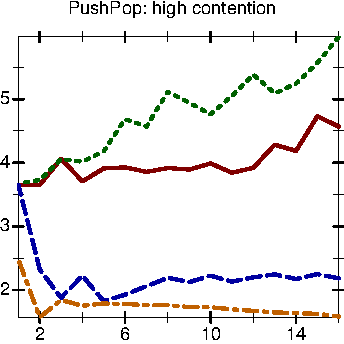
\includegraphics[scale=\gscale]{graphs/PushPop-100.pdf}
\hspace{1mm}
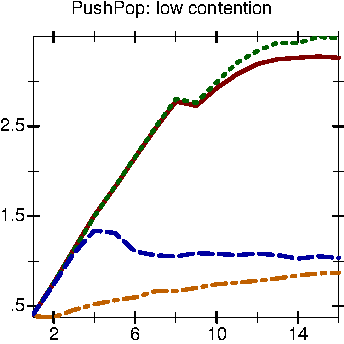
\includegraphics[scale=\gscale]{graphs/PushPop-1000.pdf}
\hspace{4mm}
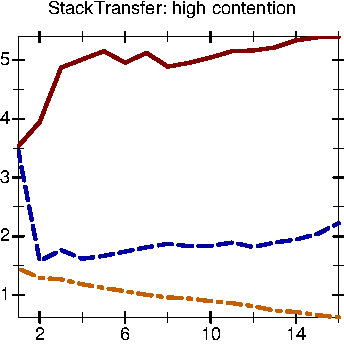
\includegraphics[scale=\gscale]{graphs/StackTransfer-100.pdf}
\hspace{1mm}
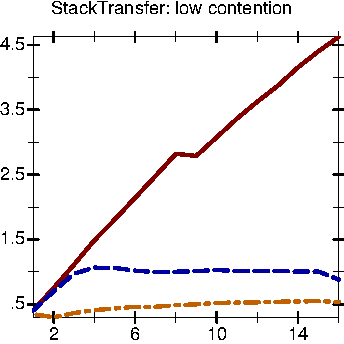
\includegraphics[scale=\gscale]{graphs/StackTransfer-1000.pdf}
\\
\\
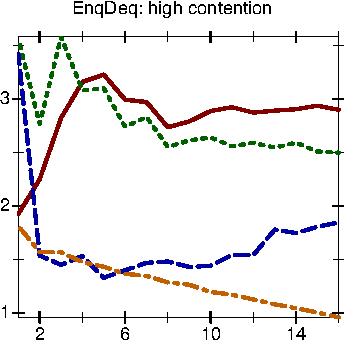
\includegraphics[scale=\gscale]{graphs/EnqDeq-100.pdf}
\hspace{1mm}
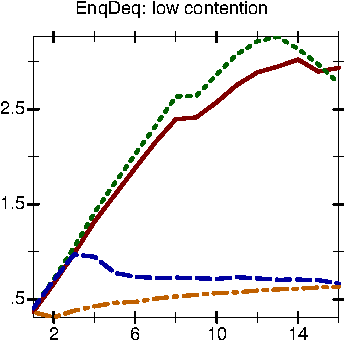
\includegraphics[scale=\gscale]{graphs/EnqDeq-1000.pdf}
\hspace{4mm}
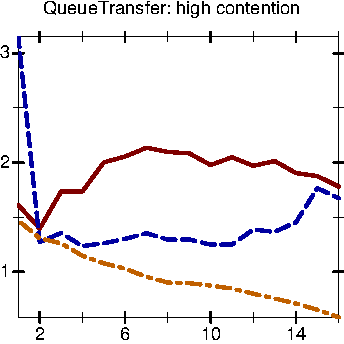
\includegraphics[scale=\gscale]{graphs/QueueTransfer-100.pdf}
\hspace{1mm}
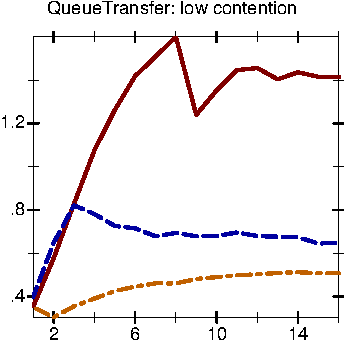
\includegraphics[scale=\gscale]{graphs/QueueTransfer-1000.pdf}
\end{tabular}
\\
& \textbf{Threads}\quad (on 16-way machine) \\
\\
& 
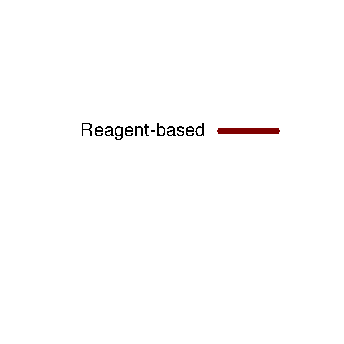
\includegraphics[scale=0.9]{graphs/reagent-based.pdf}
\qquad\qquad
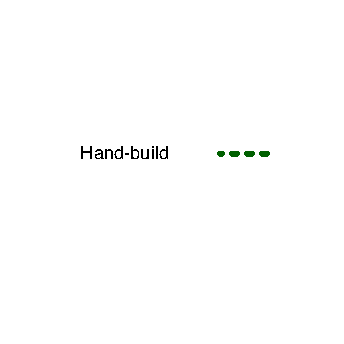
\includegraphics[scale=0.9]{graphs/hand-built.pdf}
\qquad\qquad
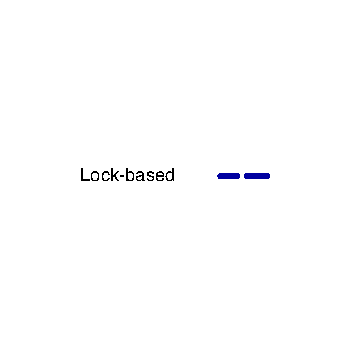
\includegraphics[scale=0.9]{graphs/lock-based.pdf}
\qquad\qquad
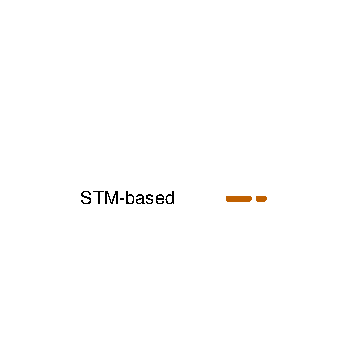
\includegraphics[scale=0.9]{graphs/stm-based.pdf}
\\
\end{tabular}
\nocaptionrule
\caption{Benchmarking results}
\label{fig:perf}
\end{figure*}

\section{Performance}
\label{sec:performance}

%\subsection{Methodology and experimental setup}

Fine-grained concurrent data structures are usually evaluated by targetted
microbenchmarking, with focus on contention effects and fine-grained parallel
speedup~\cite{Mellor-Crummey1991,Michael1996,Herlihy2003,Scherer2004,Hendler2004,Fraser2007,Cederman2010,Hendler2010}.
In addition to those basic aims, we wish to evaluate (1) the extent to which
reagent-based algorithms can compete with their hand-built counterparts and (2)
whether reagent composition is a plausible approach for scalable atomic
transfers.  To this end, we designed a series of benchmarks focusing on simple
lock-free collections, where overhead from reagents is easy to gauge.  Each
benchmark consists of $n$ threads running a loop, where in each iteration they
apply one or more atomic operations on a shared data structure and then simulate
a workload by spinning for a short time.  For a high contention simulation, the
spinning lasts for 0.25$\mu$s on average, while for a low contention simulation,
we spin for 2.5$\mu$s.

In the ``PushPop'' benchmark, all of the threads alternate pushing and popping
data to a single, shared stack.  In the ``StackTransfer'' benchmark, there are
two shared stacks, and each thread pushes to one stack, atomically transfers an
element from that stack to the other stack, and then pops an element from the
second stack; the direction of movement is chosen randomly.  The ``EnqDeq'' and
``QueueTransfer'' benchmarks are analogous, but work with queues instead.  The
stack benchmarks compare our reagent-based \lstinline{TreiberStack} to (1) a
hand-built Treiber stack, (2) a mutable stack protected by a single lock, and
(3) a stack using STM.  The queue benchmarks compare our reagent-based
\lstinline{MSQueue} to (1) a hand-built Michael-Scott queue, (2) a mutable queue
protected by a lock, and (3) a queue using STM.  For the transfer benchmarks,
the hand-built data structures are dropped, since they do not support atomic
transfer; for the lock-based data structures, we acquire both locks in a fixed
order before performing the transfer.

We used the Multiverse STM, a sophisticated open-source implementation of
Transaction Locking II~\cite{Dice2006a} which is distributed as part of the Akka
package for Scala.  Our benchmarks were run on a 3.46Ghz Intel Xeon X5677
(Westmere) with 32GB RAM and 12MB of shared L3 cache.  The machine has two
physical processors with four hyperthreaded cores each, for a total of 16
hardware threads.  L1 and L2 caches are per-core.  The software environment
includes Ubuntu 10.04.3 and the Hotspot JVM 6u27.

%\subsection{Results}

The results are shown in~\figref{perf}; the x-axes show thread counts, while the
y-axes show throughput (so larger numbers are better).  The reagent-based data
structures perform universally better than the lock- or STM-based data
structures.  The results show that reagents can plausibly competete with
hand-built concurrent data structures, while providing scalable composed
operations that are rarely provided for such data structures.

%\subsection{Potential improvements}



%%%%%%%%%%%%%%%%%%%%%%%%%%%%%%%%%%%%%%%%%%%%%%%%%%%%%%%%%%%%%%%%

\section{Related work}
\label{sec:related}

\elide{
The design of reagents builds on a foundation laid by Concurrent ML
and extended in Haskell's STM 
}

\subsection{Concurrent ML}

Concurrent ML~\cite{Reppy1991} was designed to resolve an apparent tension
between abstraction and choice: if protocols are represented abstractly as
functions, it is impossible to express the choice of two abstract protocols.
The solution is \emph{higher-order concurrency}, in which synchronous
message-passing protocols are represented abstractly as \emph{events}.  CML's
events are built up from combinators, including a choice combinator,
communication combinators, and combinators for arbitrary computations not
involving communication.  \elide{
Events are an abstract data type: externally to the
CML library, they appear as abstract, composable values.  Internally to the
library, however, events can be decomposed into their constituent combinators,
which allows CML to execute them.
}
Reagents are clearly influenced by the design of CML's events, and include
variants of CML's core event combinators\elide{(communication and choice)}.
But where CML is aimed squarely at capturing synchronous communication
protocols, reagents are designed for writing and tailoring fine-grained
concurrent data structures and synchronization primitives.  This difference in
motivation led us to include a number of additional combinators, including
those dealing directly with shared state.

Originally, CML was focused on managing concurrency rather than profiting from
parallelism, and this focus was reflected in its implementation.  More
recently, a parallel implementation of CML was proposed~\cite{Reppy2009}.  The
key challenge is resolving uses of choice both consistently and scalably.  It
is addressed by \emph{sharing}: an event making a choice is enrolled as
offering a communication corresponding to each possible choice, and when a
communication is accepted, the (single, shared) event is atomically marked as
consumed.  We follow a similar strategy in dealing with message passing, but
where Parallel CML uses lock-based queues to store messages, we show how to
use lock-free bags for increased parallelism~(\secref{implementation}).  We
also show how to incorporate choice resolution with shared-state updates and
our conjunction combinators.

\elide{
Although CML events do not form a monad~\cite{?}, the basic pattern of
representing effectful computations as abstract, composable values has become
common in monadic programming~\cite{?}, including Haskell's STM and
Transactional Events, both discussed below.
}

\subsection{Software transactional memory}
\label{sec:stm}

Software transactional memory was originally intended ``to provide a general
highly concurrent method for translating sequential object implementations into
non-blocking ones''~\cite{Shavit1997}.  This ambitious goal has led to a
remarkable research literature, which has been summarized in textbook
form~\cite{Larus2006}.  Much of the research is devoted to achieving scalability
on multiprocessors or multicores, sometimes by relaxing consistency
guarantees\elide{~\cite{?}} or only providing obstruction-freedom rather than
lock-freemdom~\cite{Herlihy2003}.  %Work in the area is

Reagents, on the other hand, are aimed at a less ambitious goal: enabling the
concise expression, user tailoring, and composition of fine-grained concurrent
algorithms.  That is, unlike STM, reagents do not attempt to provide a
\emph{universal} fine-grained concurrent algorithm.  Instead, they assist in
writing and using specific algorithms.  

There is a clear tradeoff.  Using STM, one can implement a concurrent stack or
queue by simply wrapping a sequential version in an \lstinline{atomic} block,
which requires no algorithmic insight and is simpler than the stack or queue
we give in~\secref{reagents}.  But even with a very clever STM, these
implementations are unlikely to scale as well as our elimination stack or
Michael-Scott queue; some evidence for that is shown in~\secref{performance}.

Reagents carve out a middle ground between completely hand-written algorithms
and the completely automatic \lstinline{atomic} blocks of STM.  When used in
isolation, reagents are \emph{guaranteed} to perform only the CASes that the
hand-written algorithm would, so they introduce no overhead on shared-memory
operations; by recoding an algorithm use reagents, you lose nothing.\elide{;
  we know of no STM implementation that can provide similar guarantees or a
  similar cost model} Yet unlike hand-written algorithms, reagents can be
composed using choice, tailored with new blocking behavior, or combined
into larger atomic blocks. %TODO

Haskell's STM~\cite{Harris2005a} was inspirational in showing that transactions
can be represented via monads~\cite{PeytonJones1993}, explicitly composed, and
combined with blocking and choice operators.  Reagents also form a monad, but we
have chosen an interface closer to \emph{arrows}~\cite{Hughes2000}, to encourage
static reagent layout wherever possible~(\secref{dynamic}).  Like
\lstinline{orElse} in Haskell's STM, our choice operator is left-biased.  But
unlike \lstinline{orElse}, our choice operator will attempt the right-hand side
even when the left-hand side has only failed transiently (rather than
permanently).  While the distinction appears technical, it is crucial for
supporting examples like the elimination backoff stack~(\secref{choice}).

\subsection{Transactions that communicate}

A central tenet of transactions is \emph{isolation}: transactions should not
be aware of concurrent changes to memory from other transactions.  But
sometimes it is desirable for concurrent transactions to coordinate or
otherwise communicate while executing.  Two very recent papers have proposed
mechanisms for incorporating communication with STM, in the form of
Communicating Transactions~\cite{Lesani2011} and Transaction
Communicators~\cite{Luchangco2011b}\elide{ (the latter extends earlier work on
Transaction Synchronizers~\cite{Luchangco2005})}.  In both cases, a key
question is how the expected isolation of shared memory can safely coexist
with concurrent communication.  Communicating Transactions use explicit,
asynchronous message passing to communicate; the mechanism is entirely
separate from shared memory, which retains isolation.  On the other hand,
Transaction Communicators allow isolation to be weakened in a controlled way.

Our mixture of message-passing and shared-state combinators most closely
resembles the work on Communicating Transactions.  Of course, the most important
difference is in the way we deal with shared state \elide{(and the guarantees
  provided thereby), which we} discussed in~\secref{stm}.  We also
believe that \emph{synchronous} communication is better for expressing
patterns like elimination~(\secref{choice}), since they rely on 
participants being mutually-aware.  %TODO: say more here

\elide{
There has also been work treating pure message-passing in a transactional way,
both explicitly in Transactional Events~\cite{Donnelly2006} and implicitly in
the Join Calculus~\cite{?}.  The former combines CML with an atomic sequencing
operator, while the latter introduces \emph{join patterns} that can receive
from multiple channels simultaneously and atomically.  Both are expressible
using reagents, through the combination of \lstinline{swap} and the
conjunction combinators.  Thus, reagents provide a new implementation for both
of these systems.  Previously, Transactional Events was implemented on top of
Haskell's STM, while join patterns have largely been implemented via
coarse-grained locking~\cite{?}.  
}

There has also been work treating pure message-passing in a transactional way:
Transactional Events~\cite{Donnelly2006} combines CML with an atomic
sequencing operator.  Previously, Transactional Events were implemented on top
of Haskell's STM, relied on lightweight search threads for matching
communications, and used an STM-based representation of channels.  However,
Transactional Events are expressible using reagents, through the combination
of \lstinline{swap} and the conjunction combinators.  Doing so yields a new
implementation that does not require search threads, performs parallel
matching for communication, and represents channels as lock-free bags.  We are
not in a position to do a head-to-head comparison, but based on the results
in~\secref{performance}, we expect the reagent-based implementation to scale
better on fine-grained workloads.

\subsection{Composing fine-grained concurrent data structures}

Most of the literature on fine-grained concurrent data structures is focused
on ``within-object'' atomicity, for example developing algorithms for
inserting or removing elements into a collection atomically.  However, there
has been some recent work studying the problem of transferring data atomically
between such fine-grained data structures~\cite{Cederman2010}.  The basic
approach relies on a \emph{k}CAS operation in much the same way that reagent
sequencing does.  The transfer methods must be defined manually, in advance,
and with access to the internals of the relevant data structures, whereas
reagents allow arbitrary new compositions, without manual definition, and
without access to the code or internals of the involved data structures.
Nevertheless, the implementation of reagent composition yields an algorithm
very similar to the manually-written transfer methods.

It is also possible to go in the other direction: start from STM, which
provides composition, and add an ``escape hatch'' for writing arbitrary
fine-grained concurrent algorithms within the scope of a transaction.  The
escape hatch can be provided through unlogged reads and/or writes to memory
locations being used by transactions, as in early release~\cite{Herlihy2003}
or elastic transactions~\cite{Felber2009}.  As we discussed
above~(\secref{stm}), we favor an approach where the focus is foremost on
writing fine-grained algorithms, with \emph{guarantees} about the performance
and shared-memory semantics of those algorithms.  Providing such guarantees
via an escape hatch mechanism may be difficult or impossible, depending on the
details of the STM implementation.  As we showed in~\secref{reagents}, it is
also very useful to have combinators for choice, message-passing, and
blocking, if one wishes to capture the full range of fine-grained concurrent
algorithms.

\elide{
\section{Conclusion}

We believe it is crucial to have XX, YY together

We see this work as serving the needs of two distinct groups: concurrency
experts and concurrency users.  Using reagents, experts can write libraries more
easily, because common patterns are expressible as abstractions and many are
built-in.  Users can then extend, tailor and compose the resulting library
without detailed knowledge of the algorithms involved.
}

\bibliographystyle{abbrvnat}
\bibliography{reagents}

\end{document}

# Intro notes

What do we want to accomplish?

 - motivate libraries like j.u.c
 - downsides of such libraries
   - huge research & impl effort
   - not easily extensible
   - internal structure has repeated, but unabstracted patterns
 - our contribution
   - a new way of expressing scalable algorithms that
     - doesn't lose much performance 
     - allows composition
     - is much nicer than direct programming
     - also incorporates blocking behavior

# General notes

Imposes no cache-coherence overhead on isolated data structures

Can argue that transactional-event-style liveness properties are
important if you want general way of composing fine-grained concurrent
algorithms with message-passing

To what extent do reagents encompass STM?  who are we competing with?

multiparadim, expressive, fast -- all that's great, but sales pitch
needs to be oriented around a customer with specific needs.  any
reason not to use the pitch of extensible, composable j.u.c.?

# To do

  - benchmark against STM (possibly Akka Transactors?)

  - benchmark queues, including flat combining and buckets

  - somewhere say that: we examine fairly simple examples in the
  paper, due to size constraints.  but we can handle more complex
  cases like sets/maps represented via skip lists, basket queues, 
  and are exploring flat combining.

# Outline

1.2 Title, abstract, intro,             1.0
1.0 Background                          1.0
2.5 Library overview & examples         3.0
1.5 Semantics 
1.5 Implementation/algorithms           2.2
0.5 Performance results                 1.0
1.0 Related work                        1.0
0.3 Conclusion                          0.3
0.8 Bib                                 0.5

How much time should we spend covering scalable concurrency
background?  This is perhaps tied to strategies for introducing the
library constructs: the primitives can be shown by-need for examples.
Should consult good papers like Ryan's and Jesse's for examples here.

# Semantics

Need to nail down story for overlapping state access.  In particular,
when (if ever) is an error flagged?  Unfortunately, talking about heap
unsplittability is rather more complicated than splittability.

Examples:

\begin{itemize}
\item TreiberStack
\item with blocking
\item with elimination backoff
\item MSQueue
\item with blocking
\item with buckets?
\item Counter to semaphore
\item RWLocks
\item Tree barriers
\item Dining philosophers(ish)
\item Flat combining - doesn't work if commit is two-phase process.
  probably too much to bring into scope for this paper, anyway
\end{itemize}


\elide{
\section{Semantics}
\label{sec:semantics}

Try to keep this minimal for the sake of space

Purpose of the semantics is mainly to clarify the relationship between
the shared-state and message-passing aspects of reagents.  We have
ruthlessly stripped out ...

(fractional?) permissions model

Left bias in choice operator

\begin{itemize}
  \item read, cas
  \item send
  \item choice
  \item react
  \item bind and ret
  \item computed?
\end{itemize}

Computed and lift cause problems: can potentially invoke a reagent
inside another invocation.  Just drop these.  And probably ret too.
Hmm.  This doesn't even allow us to express upd.  But upd itself is
problematic for the same reasons.

Could easily split out ``pure'' expressions.  Unsatisfying...  but
this is essentially what Haskell's STM is doing.

% NOTE: this leaves a nice opportunity later to give a full semantic
% story

\elide{
\[
\infer
  {P_i, \sigma_i \cstep{t_i} P'_i, \sigma'_i}
  {P_1 | \cdots | P_n,\ \sigma_1 \uplus \cdots \uplus \sigma_n\ \step\
   P'_1 | \cdots | P'_n,\ \sigma'_1 \uplus \cdots \uplus \sigma'_n
  }
\]

\[
\infer
  {r_i!v_i, \sigma_i \cstep{t_i} \ret{v'_i}, \sigma'_i}
  {\procCtx[\prod \evalCtx_i[r_i ! v_i]],\ \biguplus \sigma_i \step
   \procCtx[\prod \evalCtx_i[\ret{v'_i}]],\ \biguplus \sigma'_i}
\]
}

\[
\infer
  {r_i\ \lstinline{!}\ v_i, \sigma_i \cstep{t_i} \ret{v'_i}, \sigma'_i}
  {\prod \evalCtx_i[r_i ! v_i],\ \biguplus \sigma_i \step
   \prod \evalCtx_i[\ret{v'_i}],\ \biguplus \sigma'_i}
\]
}
